\documentclass[12pt,letterpaper]{article}
\usepackage{fullpage}
\usepackage[top=2cm, bottom=4.5cm, left=2.5cm, right=2.5cm]{geometry}
\usepackage{amsmath,amsthm,amsfonts,amssymb,amscd}
\usepackage{lastpage}
\usepackage{enumerate}
\usepackage{fancyhdr}
\usepackage{graphicx}


\usepackage{mathtools} % For sum thing

\setlength{\parindent}{0.0in}
\setlength{\parskip}{0.05in}


\newcommand\course{AI 701}
\newcommand\rollNumber{21010241}
\newcommand\name{Muhammad Umar Salman}

\pagestyle{fancyplain}
\headheight 35pt
\lhead{\name\\\rollNumber}

\chead{\textbf{\Large Assignment 1}}
\rhead{\course \\ \today}
\lfoot{}
\cfoot{}
\rfoot{\small\thepage}
\headsep 1.5em



\begin{document}


%%%%%%%%%%%%%%%%%%%%%%%%%%%%%%%%%%%%%%%%%%%%%%%%%%%%%%%
\section*{AI and Intelligent Agents}
\begin{enumerate}
    \item
        \begin{enumerate}
            \item \textbf{Intelligence}: Is the quality that an entity possesses so that it can perceive and reason on its own as well as behave and be self-aware according to its environment
            \item \textbf{Artificial Intelligence}:Artificial Intelligence is the intelligence given to an entity so that it can perceive and reason on its own as well as behave and be self-aware according to its environment and operate autonomously while adapting to any change.
            \item \textbf{Agent}: An agent is entity that perceives its environment through sensors and can act on its environment through actuators
            \item \textbf{Rationality}: Rationality is to act rationally. That means based on the performance measure, prior knowledge and of the environment act in the best way/ achieve the best outcome during a moment of uncertainty with whatever limited actions are available. 
            \item \textbf{Logical Reasoning}: Logical Reasoning is a way of thinking that uses deductive reasoning given a knowledge base or facts to deduce other facts by reason.
        \end{enumerate}
    \item Vision Systems are intelligent agents designed by humans to think rationally and logically as well as act in this way. But the matter of the fact is not all real-world problems can be solved on the basis of rationality and logic, humans also think instinctively. For e.g., if a person begins to think rationally or logically to remove his hand from a hot place his hand will burn by the time taken to process all the facts. So just like a human would instinctively remove his hand a human instinctively processes an image without any complex maths. This processing of images or Human "Vision Systems" can in the same way also be thought of as human instinct or human reflex. \\
    
    \item ) One of the first major successes of AI was in 1997 when IBM’s Deep Blue was the first computer program to have beat the world chess champion under regular time controls. Gary Kasparov, who had been beaten later said he felt a new type of intelligence. STANLEY, a driverless robotic car, in the 2005 DARPA Grand Challenge completed a 132-mile course at 22mph through the rough terrain of the Mojave Desert winning first prize. The following year in 2006 CMU’s BOSS won the Urban Challenge, safely driving in traffic through the streets of a closed Air Force base, obeying traffic rules and avoiding pedestrians and other vehicles. In Speech Recognition a traveler calling United Airlines to book a flight can have the entire conversation guided by an automated speech recognition and dialog management system. Launched in 1996, the Robocup Competition aims to develop a fully autonomous humanoid robots that can win against human world champion soccer team by 2050. \\
    From these 5 challenges and contests we can see that how it started from winning a chess game against a in 1997 to autonomous cars, fully conversational dialogue system which answers question to attempting to beat the world soccer champions team in a physical soccer match. From the DARPA Grand Challenge in 2005 in a empty terrain to 2006’s Urban Challenge, we can see that how much AI has progressed in the span of only a year where from empty terrain an autonomous car is driving in an urban environment with other traffic. We can also see to what degree these contests have advanced in the state-of-the-art AI when we look at the Robocup’s progress from 1996 to 2009 where 43 teams are participating in this contest and they look to robots playing against human world soccer champions by 2050. However, these contests do draw away energy from new ideas as every year each research team is trying to improve or better the AI and AI agent than last year’s winner of a certain contest rather than being innovative and creating something new that could maybe solve other problems than just working on the same thing every year.

    \item
        \begin{enumerate}
            \item \textbf{Agent}: An agent is entity that perceives its environment through sensors and can act on its environment through actuators
            \item \textbf{Agent Function}: An agent function maps a sequence of percept vectors to an action out of a set of finite actions
            \item \textbf{Agent Program}: An Agent Program is a program that runs or implements the agent function on a physical architecture (hardware + software). This program is mostly run on an artificial agent.
            \item \textbf{Rationality}:  Rationality is to act rationally. That means based on the performance measure, prior knowledge and perceptions of the environment act in the best way/ achieve the best outcome during a moment of uncertainty with whatever limited actions are available.
            \item \textbf{Autonomy}: Autonomy is the capability of taking independent actions and decision-making. That means an artificial agent  should learn from what it can from incorrect or partially incorrect prior knowledge rather than being fully dependent on that prior knowledge only.
            \item \textbf{Reflex Agent}: Reflex Agent is an agent that selects an action based on the current percept, and ignores the rest of the percept history. They are stateless agents and have no memory of past world states
        \end{enumerate}
    \item 
    \begin{enumerate}
        \item \textbf{Medical Diagnosis System}
            \begin{enumerate}
            \item Performance Measure
                \begin{enumerate}
                \item Maximize Healthiness of Patient
                \item Minimize Cost
                \item Minimize Side Effects of Treatment
                \end{enumerate}
            \item Environment
                \begin{enumerate}
                \item Patient
                \item Hospital Staff
                \item Diagnosis Room
                \end{enumerate}
            \item Sensors
                \begin{enumerate}
                \item Touch screen/Keyboard
                \item Enter Patient Answers
                \item Enter Patient Symptoms
                \end{enumerate}
            \item Actuators
                \begin{enumerate}
                \item Ask Diagnosis Questions
                \item Display Diagnosis
                \item Display Treatments
                \item Display tests to be taken
                \end{enumerate}
            \end{enumerate}
        \item \textbf{Satellite Image Analysis System}
            \begin{enumerate}
            \item Performance Measure
                \begin{enumerate}
                \item Maximize Classification Accuracy
                \item Minimize computation time
                \item Maximize Image Quality
                \end{enumerate}
            \item Environment
                \begin{enumerate}
                \item Outer Space
                \item Satellite
                \item Downlink from satellite
                \end{enumerate}
            \item Sensors
                \begin{enumerate}
                \item Camera
                \item Color pixel array
                \end{enumerate}
            \item Actuators
                \begin{enumerate}
                \item Image Capturer (Takes Images)
                \item Display Classification
                \end{enumerate}
            \end{enumerate}
        \item \textbf{Interactive English Tutor}
            \begin{enumerate}
            \item Performance Measure
                \begin{enumerate}
                \item Improve Students English
                \item Maximize students score
                \item Minimize English mistakes
                \end{enumerate}
            \item Environment
                \begin{enumerate}
                \item Students
                \item Mock Tests
                \item Testing Agency
                \end{enumerate}
            \item Sensors
                \begin{enumerate}
                \item Keyboard/Touch Screen
                \item Mic for Vocal Answers
                \item Student Answers
                \end{enumerate}
            \item Actuators
                \begin{enumerate}
                \item Display Corrections
                \item Display Mock Questions
                \item Display Suggestions
                \end{enumerate}
            \end{enumerate}
    \end{enumerate}
\end{enumerate}

%%%%%%%%%%%%%%%%%%%%%%%%%%%%%%%%%%%%%%%%%%%%%%%%%%%%%%%
\section*{Calculus Recap}
    \begin{enumerate}
            \item $3x^2 + 1$
            \item 
                $f( \theta ) =  \frac{1}{2} \sum_{i=1}^{n}  w_{i}(\theta -  x_{i})^2$  \\ \\
                $\frac{d(f(\theta)) }{d\theta} =  \frac{1}{2}  \sum_{i=1}^{n}  2w_{i}(\theta -  x_{i})^{2-1} \cdot 1$ \\ \\
                $\frac{d(f(\theta)) }{d\theta} =  \sum_{i=1}^{n}  w_{i}(\theta -  x_{i}) \\ \\$
                To minimize $\theta: \frac{d(f(\theta)) }{d\theta} = 0$
                $\sum_{i=1}^{n}  w_{i}(\theta -  x_{i}) = 0 \\ \\$
                $\sum_{i=1}^{n}  (\theta w_{i} -  x_{i}w_{i}) = 0 \\ \\$
                $\sum_{i=1}^{n} \theta w_{i} -  \sum_{i=1}^{n} x_{i}w_{i} = 0 \\ \\ $
                $\sum_{i=1}^{n} \theta w_{i} =  \sum_{i=1}^{n} x_{i}w_{i}\\ \\$
                $\theta \sum_{i=1}^{n} w_{i} =  \sum_{i=1}^{n} x_{i}w_{i}\\ \\$
                $\theta =  \frac{\sum_{i=1}^{n} x_{i}w_{i}}{\sum_{i=1}^{n} w_{i}}\\ \\$
            \item 
                $f(w) = \sum_{i=1}^{n} \sum_{j=1}^{n} (a_{i}^Tw - b_{i}^Tw)^2 +  \lambda  \parallel w \parallel_{2}^2$ \\ \\
                $f(w) = \\ (a_{1}^Tw - b_{1}^Tw)^2 + (a_{1}^Tw - b_{2}^Tw)^2 + ... + (a_{1}^Tw - b_{n}^Tw)^2$ \\
                $(a_{2}^Tw - b_{1}^Tw)^2 + (a_{2}^Tw - b_{2}^Tw)^2 + ... + (a_{2}^Tw - b_{n}^Tw)^2 $\\
                : \\
                : \\
                $(a_{n}^Tw - b_{1}^Tw)^2 + (a_{n}^Tw - b_{2}^Tw)^2 + ... + (a_{n}^Tw - b_{n}^Tw)^2 + \lambda  \parallel w \parallel_{2}^2$ \\ \\
                
                $\frac{df(w)}{w} = \\ \\ 2(a_{1}^Tw - b_{1}^Tw)(a_{1} - b_{1}) + 2(a_{1}^Tw - b_{2}^Tw)(a_{1} - b_{2}) + ... + 2(a_{1}^Tw - b_{n}^Tw)(a_{1} - b_{n})$ \\
                $2(a_{2}^Tw - b_{1}^Tw)(a_{2} - b_{1}) + 2(a_{2}^Tw - b_{2}^Tw)(a_{2} - b_{2}) + ... + 2(a_{2}^Tw - b_{n}^Tw)(a_{2} - b_{n}) $\\
                : \\
                : \\
                $2(a_{n}^Tw - b_{1}^Tw)(a_{n} - b_{1}) + 2(a_{n}^Tw - b_{2}^Tw)(a_{n} - b_{2}) + ... + 2(a_{n}^Tw - b_{n}^Tw)(a_{n} - b_{n}) +  \frac{d(\lambda  \parallel w \parallel_{2}^2)}{dw} $ \\ \\
                \textbf{Solving Lambda Term} $ \frac{d(\lambda  \parallel w \parallel_{2}^2)}{dw}:$ \\ \\
                $ lambda  \parallel w \parallel_{2}^2  = \lambda (( \sum_{k=1}^{n} w^2)^{1/2})^{2})$ \\ \\
                $ lambda  \parallel w \parallel_{2}^2  =\lambda( \sum_{k=1}^{n} w^2)$ \\ \\
                $ \frac{d(\lambda  \parallel w \parallel_{2}^2)}{dw}  =2 \lambda \sum_{k=1}^{n} w$ \\ \\
                $ \frac{d(\lambda  \parallel w \parallel_{2}^2)}{dw}  = 2 \lambda w$ \\
                
                \textbf{Thus Solving} \\
                
                $ \frac{df(w)}{w} = \sum_{i=1}^{n} \sum_{j=1}^{n} (a_{i}^Tw - b_{i}^Tw)(a_{i} - b_{j}) + 2 \lambda w $
    \end{enumerate}
%%%%%%%%%%%%%%%%%%%%%%%%%%%%%%%%%%%%%%%%%%%%%%%%%%%%%%%
\section*{Linear Algebra Warm Up}
    \begin{enumerate}
            \item
            \begin{enumerate}
                \item $y^T z = (1\cdot2) + (3\cdot3) = 11$
                \item $Xy = \begin{bmatrix}(2\cdot1) + (4\cdot3) \\(1\cdot1) + (3\cdot3)\end{bmatrix} = \begin{bmatrix}14 \\ 10 \end{bmatrix}$
                \item 
                Yes X is invertible because it is a square matrix and has a determinant which is not equal to 0 \\
                $X^{-1} =  \frac{1}{(2\cdot3) + (-1\cdot-4)}  \begin{bmatrix}3 & -4 \\ -1 & 2 \end{bmatrix} =  \begin{bmatrix}1.5 & -2 \\ -0.5 & 1 \end{bmatrix}$
                \item
                The rank of a matrix is the maximum number of its linearly independent column vectors or row vectors. This can be found by counting the number of non-zero rows or non-zero columns. Therefore, if we have to find the rank of a matrix, we will transform the given matrix to its row echelon form and then count the number of non-zero rows.
                
                First we reduce matrix to row echelon form = $\begin{bmatrix}2 & 4 \\ 0 & 3 \end{bmatrix}$ \\
                Then calculate the number of linearly independent rows = 2 
                \\
                Thus, Rank of Matrix X = 2
            \end{enumerate}
            \item
            \textbf{Orthognal}: A square matrix with real numbers or elements is said to be an orthogonal matrix, if its transpose is equal to its inverse matrix. Or we can say, when the product of a square matrix and its transpose gives an identity matrix, then the square matrix is known as an orthogonal matrix
            \item
            \textbf{Positive Semi Definite}: Matrix A is a positive semi-definite if it is a Hermitian matrix whose eigen values are non negative
            
            \item
            \textbf{Psuedo Inverse}: The pseudo-inverse is defined and unique for all matrices whose entries are real or complex numbers. It is a generalization of the matrix inverse when a matrix isn't invertible and it does this through singular value decomposition.
            
    \end{enumerate}

%%%%%%%%%%%%%%%%%%%%%%%%%%%%%%%%%%%%%%%%%%%%%%%%%%%%%%%
\section*{Probability and Statistics Recap}
    \begin{enumerate}
            \item 
            Sample Mean = $ \frac{1+1+0+1+0}{5} =  \frac{3}{5} $
            \item
            Sample variance = $S^2$ \\ \\
            $S^2 =  \frac{1}{n}  \sum_{i=-1}^{n} (x_{i} -  \overline{x})^2$  \\ \\
            $= \frac{1}{5} \begin{bmatrix}(\frac{2}{5})^2 + (\frac{2}{5})^2 + (-\frac{3}{5})^2 + (\frac{2}{5})^2 + (-\frac{3}{5})^2\end{bmatrix}$  \\ \\
            $= \frac{1}{5}  \begin{bmatrix} \frac{3\cdot4}{25} +  \frac{2\cdot9}{25} \end{bmatrix}$  \\ \\
            $=  \frac{6}{25}$
            \item
            $P(S) = 0.5^5 =  \frac{1}{32}$ 
    \end{enumerate}

%%%%%%%%%%%%%%%%%%%%%%%%%%%%%%%%%%%%%%%%%%%%%%%%%%%%%%%
\section*{Machine Learning}
    \begin{enumerate}
            \item 
                \begin{enumerate}
                    \item
                    $ Loss(x,y,w) =  (\sigma (w. \phi (x)) - y)^2$ \\ \\
                    $Loss(x,y,w) = ( \frac{1}{1+ e^{-w. \phi (x)}} - y )^2$ \\
                    \item 
                    $Loss(x,y,w) = (\sigma (w. \phi (x)) - y)^2 = ( \frac{1}{1+ e^{-w. \phi (x)}} - y )^2$ \\ \\
                    Let p = $\sigma (w. \phi (x))  \Rightarrow Loss(x,y,z) = (p - y)^2$ \\ \\
                    $\frac{d(Loss(x,y,z))}{dw} = \frac{(p - y)^2}{dw}  = 2(p-y) \frac{d(p)}{dw}$ \\ \\
                    Solving for $\frac{d(p)}{dw}:$ \\ \\
                    $\frac{d(p)}{dw} =  \frac{d(\begin{bmatrix} 1+ e^{-w. \phi (x)} \end{bmatrix}^{-1} )}{dw} = -1(\frac{1}{1+ e^{-w. \phi (x)}})^{-2}\cdot (-\phi (x)\cdot  e^{-w. \phi (x)}) \;\;\;\; \vdots \vdots \vdots \;\;\;\;  \frac{d(e^{ax})}{dx} = ae^{ax}$ \\ \\
                    $\frac{d(p)}{dw} = \phi (x)(\frac{1}{1+ e^{-w. \phi (x)}})^{-2}\cdot (e^{-w. \phi (x)}) = \phi (x)  \begin{bmatrix}\frac{1}{1+ e^{-w. \phi (x)}} \cdot \frac{e^{-w. \phi (x)}}{1+ e^{-w. \phi (x)}}\end{bmatrix}$ \\ \\
                    $\frac{d(p)}{dw} = \phi (x)  \begin{bmatrix}\frac{1}{1+ e^{-w. \phi (x)}} \cdot \frac{1 + e^{(-w. \phi (x))}  -1}{1+ e^{-w. \phi (x)}}\end{bmatrix} = \phi (x)  \begin{bmatrix}\frac{1}{1+ e^{-w. \phi (x)}} \cdot (1 - \frac{1}{1+ e^{-w. \phi (x)}}) \end{bmatrix}$ \\ \\
                    $ \frac{d(p)}{dw} = \phi (x)p(1-p)$ \\ \\
                    Substituting $ \frac{d(p)}{dw}$ \\ \\
                    $\frac{d(Loss(x,y,z))}{dw} = 2\phi(x)(p-y)p(1-p)$ \\ \\
                    
                    \item 
                    We know that the gradient of the loss with respect to w is: \\ \\
                    $\frac{d(Loss(x,y,z))}{dw} = 2\phi(x)(p-y)p(1-p)$ , where p = $\frac{1}{1+ e^{-w. \phi (x)}}$ \\ \\
                    Lets call z = $w. \phi (x)$. If we assume that y = 1 then the value of p that makes the magnitude of the gradient of loss arbitrarily small is p approaching 1. As p approaches 1 the gradient of loss becomes arbitrarily small because of (p-y) and (1-p). We know that p is the sigmoid function which depends on the value of z. As z increases to an arbitrarily large number p approaches 1. And since z is directly proportional to w, that means as the value of w increases to an arbitrarily large number so does z, causing p to approach 1 which causes the gradient of the loss function to become arbitrarily small.Thus the condition for w would be to become arbitrarily large to make the magnitude extremely small.This value of the gradient of the loss function can go extremely small as the magnitude of w increases but can not become 0 as the sigmoid function has two horizontle asymptotes at y=0 and y=1. So p can approach 1 but can never equal 1 thus the gradient can never be exactly 0. 
                    
                    \begin{figure}[!h]
                    \centering
                    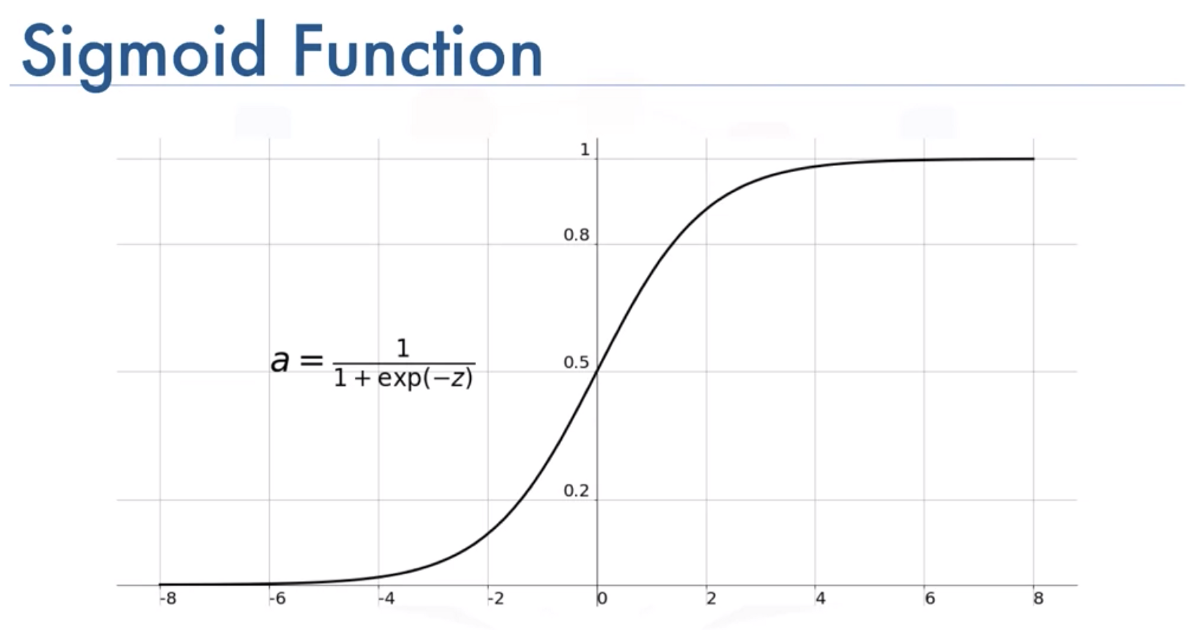
\includegraphics[width=0.3\linewidth]{Sigmoid.png}
                    \caption{Image of the Sigmoid Function.}
    \end{figure}
                \end{enumerate}
            \item True
            \item
                \begin{enumerate}
                    \item 
                    Points: \\
                    $\phi (x_{1}) = \begin{bmatrix}1, 0 \end{bmatrix} $\\
                    $\phi (x_{2}) = \begin{bmatrix}1, 2 \end{bmatrix} $\\
                    $\phi (x_{3}) = \begin{bmatrix}3, 0 \end{bmatrix} $\\
                    $\phi (x_{4}) = \begin{bmatrix}2,2 \end{bmatrix} $\\ \\
                    \textbf{Running with First Centres:} \\ \\
                    First Run ... \\
                    \textit{Assign Members}
                    With centres  $\mu_{1} =  \begin{bmatrix}2, 3\end{bmatrix}$  and $\mu_{2} = \begin{bmatrix}2, -1\end{bmatrix}$ \\ \\
                    Euclidean Distance Squared for $\phi (x_{1})$ to $\mu_{1} = 10 $ and $\mu_{2} = 2$ \\
                    Assigned to: Group 2 \\
                    Euclidean Distance Squared for $\phi (x_{1})$ to $\mu_{1} = 2 $ and $\mu_{2} = 10$ \\
                    Assigned to: Group 1 \\
                    Euclidean Distance Squared for $\phi (x_{1})$ to $\mu_{1} = 10 $ and $\mu_{2} = 2$ \\
                    Assigned to: Group 2 \\
                    Euclidean Distance Squared for $\phi (x_{1})$ to $\mu_{1} = 1 $ and $\mu_{2} = 9$ \\
                    Assigned to: Group 1 \\ \\
                    \textit{Update Centers} \\
                    $\mu_{1} = average(\phi (x_{2}, \phi (x_{4}) =  \begin{bmatrix} 1.5, 2.0 \end{bmatrix} $ \\
                    $\mu_{2} = average(\phi (x_{1}, \phi (x_{3}) =  \begin{bmatrix} 2.0, 0.0 \end{bmatrix}$ \\ \\
                    
                    Second Run ... \\
                    \textit{Assign Members}
                    With centres  $\mu_{1} =  \begin{bmatrix}1.5, 2.0\end{bmatrix}$  and $\mu_{2} = \begin{bmatrix}2.0, 0.0\end{bmatrix}$ \\ \\
                    Euclidean Distance Squared for $\phi (x_{1})$ to $\mu_{1} = 4.25 $ and $\mu_{2} = 1$ \\
                    Assigned to: Group 2 \\
                    Euclidean Distance Squared for $\phi (x_{1})$ to $\mu_{1} = 0.25 $ and $\mu_{2} = 5$ \\
                    Assigned to: Group 1 \\
                    Euclidean Distance Squared for $\phi (x_{1})$ to $\mu_{1} = 6.25 $ and $\mu_{2} = 1$ \\
                    Assigned to: Group 2 \\
                    Euclidean Distance Squared for $\phi (x_{1})$ to $\mu_{1} = 0.25 $ and $\mu_{2} = 4$ \\
                    Assigned to: Group 1 \\ \\
                    \textit{Final Centers} \\
                    $\mu_{1} = average(\phi (x_{2}, \phi (x_{4}) =  \begin{bmatrix} 1.5, 2.0 \end{bmatrix} $ \\
                    $\mu_{2} = average(\phi (x_{1}, \phi (x_{3}) =  \begin{bmatrix} 2.0, 0.0 \end{bmatrix}$ \\ \\
                    
                    \textbf{Running with Second Centres:} \\ \\
                    First Run ... \\
                    \textit{Assign Members} With centres  $\mu_{1} =  \begin{bmatrix}0, 1\end{bmatrix}$  and $\mu_{2} = \begin{bmatrix}3, 2\end{bmatrix}$ \\ \\
                    uclidean Distance Squared for $\phi (x_{1})$ to $\mu_{1} = 2 $ and $\mu_{2} = 8$ \\
                    Assigned to: Group 1 \\
                    Euclidean Distance Squared for $\phi (x_{1})$ to $\mu_{1} = 2 $ and $\mu_{2} = 4$ \\
                    Assigned to: Group 1 \\
                    Euclidean Distance Squared for $\phi (x_{1})$ to $\mu_{1} = 10 $ and $\mu_{2} = 4$ \\
                    Assigned to: Group 2 \\
                    Euclidean Distance Squared for $\phi (x_{1})$ to $\mu_{1} = 5 $ and $\mu_{2} = 1$ \\
                    Assigned to: Group 2 \\ \\
                    \textit{Update Centers} \\
                    $\mu_{1} = average(\phi (x_{2}, \phi (x_{4}) =  \begin{bmatrix} 1.0, 1.0 \end{bmatrix} $ \\
                    $\mu_{2} = average(\phi (x_{1}, \phi (x_{3}) =  \begin{bmatrix} 2.5, 1.0 \end{bmatrix}$ \\ \\
                    
                    Second Run ... \\
                    \textit{Assign Members}
                    With centres  $\mu_{1} =  \begin{bmatrix}1.0, 1.0\end{bmatrix}$  and $\mu_{2} = \begin{bmatrix}2.5, 1.0\end{bmatrix}$ \\ \\
                    Euclidean Distance Squared for $\phi (x_{1})$ to $\mu_{1} = 1 $ and $\mu_{2} = 3.25$ \\
                    Assigned to: Group 1 \\
                    Euclidean Distance Squared for $\phi (x_{1})$ to $\mu_{1} = 1 $ and $\mu_{2} = 3.25$ \\
                    Assigned to: Group 1 \\
                    Euclidean Distance Squared for $\phi (x_{1})$ to $\mu_{1} = 5 $ and $\mu_{2} = 1.25$ \\
                    Assigned to: Group 2 \\
                    Euclidean Distance Squared for $\phi (x_{1})$ to $\mu_{1} = 2 $ and $\mu_{2} = 1.25$ \\
                    Assigned to: Group 2 \\ \\
                    \textit{Final Centers} \\
                    $\mu_{1} = average(\phi (x_{2}, \phi (x_{4}) =  \begin{bmatrix} 1.0, 1.0 \end{bmatrix} $ \\
                    $\mu_{2} = average(\phi (x_{1}, \phi (x_{3}) =  \begin{bmatrix} 2.5, 1.0 \end{bmatrix}$ \\ \\
                    
                    
                    \item Running K-Means multiple times on the same dataset with different random initializations gives a higher probability of converging to a global minima rather than doing it with one initialization which most probably converges to local minima.

                    \item No, because K Means is very sensitive to scaling and will give more weightage to the features with the larger variances. This will cause the larger variance feature to be more affected by the Euclidean distance causing the assignment of each cluster to be affected by the larger variance feature. Thus giving different clusters before and after scaling. This would also be true if we only scaled only dimensions as well.
                \end{enumerate}
             
    \end{enumerate}

\end{document}
